W~zaproponowanym algorytmie wykrywania logo \bk, można wydzielić pięć odrębnych faz przetwarzania. Poszczególne fazy zostały zaprezentowane za pomocą schematu blokowego na rysunku~\ref{fig:algorithm-overview}.

\begin{figure}
    \centering
    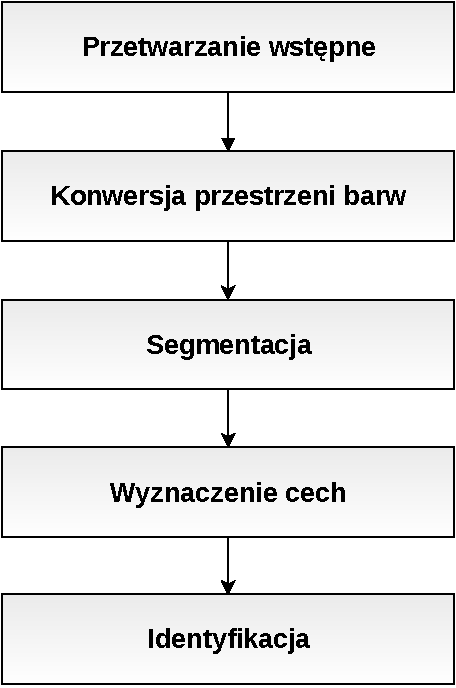
\includegraphics[width=0.6\columnwidth]{figures/algorithmOverview.pdf}
    \caption{Ogólny schemat blokowy algorytmu wykrywania logo \bk}
    \label{fig:algorithm-overview}
\end{figure}

W~pierwszej kolejności obraz zostanie przepuszczony przez moduł przetwarzania wstępnego. Jego zadaniem jest poprawa jakości obrazu oraz ujednolicenie jego rozmiaru.
Następnie obraz zostanie przekonwertowany do odpowiedniej przestrzeni barw, tak aby móc przeprowadzić proces segmentacji obrazu. Dla każdego wykrytego segmentu, wyznaczone zostanie dla niego zestaw cech, na podstawie których przeprowadzony zostanie etap identyfikacji.

\subsection{Szczegóły implementacyjne}
Cały algorytm wykrywania został zaimplementowany przy pomocy języka C++. Program korzysta ze specjalnie przygotowanych klas i~narzędzi, realizujących podstawowe algorytmy przetwarzania obrazu, zagregowanych w~pakiecie \texttt{POBR}. Akwizycja obrazu, jego wyświetlanie, zapisywanie oraz przechowywanie w~pamięci zostało zrealizowane za pomocą biblioteki OpenCV~\cite{opencv}. Aplikacja korzysta z~szeregu parametrów, które są wczytywane z~pliku konfiguracyjnego w~formacie YAML~\cite{swierczynski2008podwyzszanie}.
